% Exact visual transcription of Xi Yin, Physics 253a, original note pp. 1--9.
% Combined source PDF: physical pp. 6--14.
% Source SHA-256: 9e5e4d241fffffa56c1c3df6dce4b83178f75787dd5d794a18c5d0c087769f21
%
% Transcription policy:
% - Page boundaries, source order, bullets, dashes, arrows, marginalia, and
%   meaningful ink colors are retained.
% - Spelling and abbreviations follow the handwritten source.
% - Mathematical expressions are not normalized silently.
% - Entries marked AMBIGUITY are discussed in ambiguities.md.
% - This is a source-layer fragment, not edited textbook prose.
%
% Compilation requirements for the reconstructed diagrams and annotations:
%   xcolor, tikz, tikz libraries arrows.meta, positioning,
%   and decorations.pathmorphing.

\providecommand{\YinPageBoundary}[2]{%
  \clearpage
  \noindent\textsf{[Original Physics 253a note p.~#1; combined PDF physical p.~#2]}%
  \par\medskip
}
\providecommand{\YinLine}[1]{\noindent #1\par}
\providecommand{\YinIndent}[1]{\noindent\hspace*{2em}#1\par}
\providecommand{\YinBullet}[1]{\noindent\hspace*{1em}$\bullet$\hspace{0.7em}#1\par}
\providecommand{\YinDash}[1]{\noindent\hspace*{1em}--\hspace{0.7em}#1\par}
\providecommand{\YinBlue}[1]{{\color[rgb]{0.00,0.34,0.92}#1}}
\providecommand{\YinLightBlue}[1]{{\color[rgb]{0.47,0.67,0.82}#1}}
\providecommand{\YinPurple}[1]{{\color[rgb]{0.61,0.16,0.88}#1}}
\providecommand{\YinGray}[1]{{\color[rgb]{0.58,0.58,0.58}#1}}
\providecommand{\YinGreen}[1]{{\color[rgb]{0.00,0.52,0.22}#1}}
\providecommand{\YinRed}[1]{{\color[rgb]{0.95,0.18,0.10}#1}}
\providecommand{\ket}[1]{\lvert #1\rangle}
\providecommand{\bra}[1]{\langle #1\rvert}
\providecommand{\braket}[2]{\langle #1\mid #2\rangle}

% ---------------------------------------------------------------------------
\YinPageBoundary{1}{6}

\YinLine{Q: What is QFT?}

% The rest of the page is one branching diagram. Text placement and colored
% course arrows are reconstructed below.
\begin{center}
\begin{tikzpicture}[
  >=Stealth,
  every node/.style={font=\small},
  branch/.style={line width=0.75pt},
  coursea/.style={->,draw=blue,line width=1.0pt},
  courseb/.style={->,draw=violet,line width=1.0pt}
]
  \node (answer) at (0,0) {A: QM $+$ locality};
  \node[anchor=north,align=center] (local-title) at (-4.2,-1.5)
    {local \YinGray{(``UV complete'')}\\QFT};
  \node[anchor=north,align=center] (eft-title) at (4.2,-1.5)
    {Effective field Theory};
  \draw[branch] (answer.south) -- (-4.2,-1.25);
  \draw[branch] (answer.south) -- (4.2,-1.25);
  \draw[blue,dashed,line width=0.7pt] (0,-1.55) -- (0,-11.7);

  \node[anchor=north west,align=left,text width=6.9cm] at (-7.6,-2.5) {%
    $\bullet$ QM w/ Poincar\'e sym\\[-1pt]
    \hspace*{1.2em}\YinGray{(and necessarily $\infty$-ly\\
    \hspace*{2.2em}many d.o.f.)}\\[5pt]
    $\bullet$ local ``field'' operators\\[5pt]
    $\bullet$ micro causality\\[8pt]
    Examples:\\[4pt]
    \hspace*{1.2em}$\bullet$ $\phi^4$ theory in $D=2,3$\\[8pt]
    \hspace*{1.2em}$\bullet$ Statistical Ising model\\
    \hspace*{2.6em}in $D=2,3$ near\\
    \hspace*{2.6em}criticality\\[8pt]
    \hspace*{1.2em}$\bullet$ Yang--Mills / QCD
  };

  \node[anchor=north west,align=left,text width=6.7cm] at (0.5,-2.5) {%
    $\bullet$ defined perturbatively\\
    \hspace*{1.2em}based on a path integral\\
    \hspace*{1.2em}over space of fields\\[5pt]
    $\bullet$ captures long-distance\\
    \hspace*{1.2em}low-energy observables
  };

  \node[draw={rgb,1:red,0.47;green,0.67;blue,0.82},
        anchor=north west,align=left,text width=6.0cm,
        minimum height=3.6cm,inner sep=7pt] (ren) at (0.55,-5.8) {%
    $\bullet$ $\phi^4$ theory in $D=4$\\[6pt]
    $\bullet$ QED\\[6pt]
    $\bullet$ standard model.
  };
  \node[anchor=south,inner sep=1pt,text={rgb,1:red,0.47;green,0.67;blue,0.82}]
    at (ren.north) {renormalizable};

  \node[draw=violet,anchor=north west,align=left,text width=6.0cm,
        minimum height=2.6cm,inner sep=7pt] (nonren) at (0.75,-10.0) {%
    $\bullet$ chiral perturbation theory\\[8pt]
    $\bullet$ GR
  };
  \node[anchor=north,text=violet] at (3.8,-12.75) {non-renormalizable};

  \node[text=blue] (a253) at (-0.75,-5.55) {253a};
  \draw[coursea] (a253.west) to[bend left=18] (-2.3,-5.9);
  \draw[coursea] (a253.east) to[bend left=10] (1.2,-6.4);
  \draw[coursea] (a253.south east) to[bend right=10] (1.3,-7.45);

  \node[text=violet] (b253) at (-0.75,-10.25) {253b};
  \draw[courseb] (b253.west) to[bend right=18] (-2.3,-8.6);
  \draw[courseb] (b253.north west) to[bend right=15] (-2.3,-7.25);
  \draw[courseb] (b253.east) to[bend left=12] (1.3,-10.55);
\end{tikzpicture}
\end{center}

% ---------------------------------------------------------------------------
\YinPageBoundary{2}{7}

\begin{center}
  \underline{Plan of 253a}
\end{center}

\YinLine{(1)\quad Lagrangian formulation of QM}
\YinBullet{path integral, regularization}
\YinBullet{perturbation theory, Feynman diagrams}
\YinBullet{renormalization and counter terms}

\bigskip
\YinLine{(2)\quad Relativistic particles and fields}
\YinBullet{$\phi^4$ theory}
\YinBullet{Green functions}
\YinBullet{asymptotic states}
\YinBullet{S-matrix, LSZ reduction}

\bigskip
\YinLine{(3)\quad Particles and fields with spin}
\YinBullet{classification of relativistic particles}
\YinBullet{fermions and gauge bosons}
\YinBullet{QED}
\YinBullet{Applications: electron $g$-factor,\\
  \hspace*{1.4em}Lamb shift.}

% ---------------------------------------------------------------------------
\YinPageBoundary{3}{8}

\YinLine{Prelude: why do we need}
\YinIndent{``field theory'' to describe QM of}
\YinIndent{particles with relativistic symmetry?}

\bigskip
\YinBullet{Hilbert space $\mathcal H$}
\YinIndent{--\quad vacuum $\ket{\Omega}$, \quad $H\ket{\Omega}=0$.}
\YinIndent{$\bullet$\quad single particle $\ket{\vec p}$%
  \hfill\YinGray{$p^\mu\equiv(p^0,\vec p)$}}
\YinLine{\hfill\YinGray{$D$-dimensional}\hspace*{2em}}
\[
  H\ket{\vec p}=\sqrt{\vec p^{\,2}+m^2}\,\ket{\vec p}.
\]
\YinIndent{$\bullet$\quad multi-particle
  $\ket{\vec p_1,\ldots,\vec p_n}$}
\YinIndent{\hspace*{2.5em}(non-interacting)}
\[
  H=\sum_{i=1}^{n}\sqrt{\vec p_i^{\,2}+m^2}.
\]

\YinLine{Equivalently, we can introduce}
\[
\left.
\begin{array}{r@{\quad}c}
  \text{creation}     & a_{\vec p}^{+}\\[3pt]
  \text{annihilation} & a_{\vec p}
\end{array}
\right\}\quad\text{operators.}
\]
\[
  \ket{\vec p}=a_{\vec p}^{+}\ket{\Omega}.
\]

% ---------------------------------------------------------------------------
\YinPageBoundary{4}{9}

\[
  \ket{\vec p_1,\vec p_2}
  =a_{\vec p_1}^{+}a_{\vec p_2}^{+}\ket{\Omega},
  \qquad \text{etc.}
\]
\[
  [a,a]=[a^{+},a^{+}]=0,
\]
\[
  [a_{\vec p},a_{\vec p'}^{+}]
  =\delta^{(D-1)}(\vec p-\vec p'),
\]
\YinGray{%
\[
  \text{so that}\qquad
  \braket{\vec p}{\vec p'}=\delta^{(D-1)}(\vec p-\vec p')
\]
}

\YinLine{We can then express the Hamiltonian as}
\[
  H=\int d^{D-1}\vec p\,
  \sqrt{\vec p^{\,2}+m^2}\,
  a_{\vec p}^{+}a_{\vec p}.
\]
\YinDash{a QM system of free relativistic}
\YinIndent{\hspace*{1.4em}particles.}
\begin{center}
  \YinBlue{$\checkmark$}
\end{center}

\YinDash{What about interacting particles?}
\[
  \begin{tikzpicture}[baseline=(prefix.base)]
    \node[inner sep=0pt] (prefix) {$H=H_0+$};
    \node[anchor=base west,inner sep=0pt] (hint) at (prefix.base east)
      {$H_{\mathrm{int}}$};
    \node[text=blue,below=11mm of hint,inner sep=0pt] (terms)
      {$a^{+}a^{+}a,\quad aaa^{+},\quad\ldots$};
    \draw[blue,line width=0.85pt]
      (hint.south west) .. controls +(0,-5mm) and +(0,-5mm) ..
      (hint.south east);
  \end{tikzpicture}
\]
\YinDash{not easy to find $H_{\mathrm{int}}$ that}
\YinIndent{\hspace*{1.4em}respects relativistic symmetry!}

% ---------------------------------------------------------------------------
\YinPageBoundary{5}{10}

\YinLine{Issue: \qquad Causality}

% Spacetime/lightcone diagram reconstructed from the source.
\begin{center}
\begin{tikzpicture}[>=Stealth,scale=0.90,every node/.style={font=\small}]
  \draw[->,line width=0.75pt] (-3.2,0) -- (4.8,0)
    node[right] {space $\vec x$};
  \draw[->,line width=0.75pt] (-2.2,-1.5) -- (-2.2,4.0)
    node[above] {time $x^0$};
  \draw[green!60!black,line width=1.15pt]
    (-0.1,0) .. controls (-0.75,0.75) and (-1.2,1.25) .. (-2.0,3.4);
  \draw[green!60!black,line width=1.15pt] (-0.1,0) -- (2.1,3.7)
    node[above right,text=green!60!black] {lightcone};
  \draw[green!60!black,line width=1.15pt] (-0.1,0) -- (-1.9,-2.0);
  \draw[green!60!black,line width=1.15pt] (-0.1,0) -- (2.3,-2.5);
  \fill[blue] (-0.1,0) circle (2.5pt);

  \draw[violet,dashed,line width=1.0pt] (-0.1,0) -- (0.55,2.85);
  \draw[violet,->,line width=1.0pt] (0.14,1.05) -- (0.28,1.65);
  \fill[violet] (0.55,2.85) circle (3pt);
  \draw[red,dashed,line width=1.0pt] (-0.1,0) -- (2.75,2.2);
  \draw[red,->,line width=1.0pt] (0.85,0.73) -- (1.48,1.22);
  \fill[red] (2.75,2.2) circle (3pt);
  \node[anchor=west,align=left] at (3.15,2.3)
    {super-luminal\\propagation forbidden!};
\end{tikzpicture}
\end{center}

\YinLine{In a generic QM system,}
\YinLine{signal propagation can be instantaneous
  $\ldotp\ldotp\ldotp\ldotp$}

\bigskip
\YinLine{In a relativistic system, expect}
\YinIndent{local disturbance to be represented by}
\begin{center}
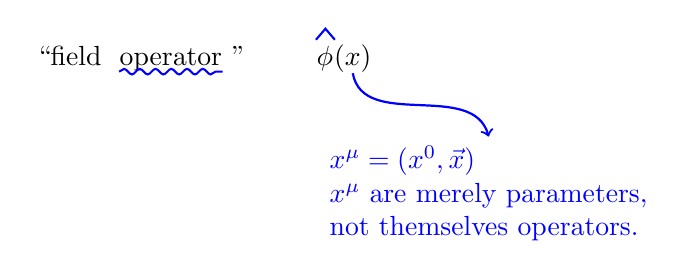
\begin{tikzpicture}[every node/.style={font=\normalsize}]
  \node[anchor=base east] (fieldword) at (-0.6,0) {``field};
  \node[anchor=base west,inner sep=0pt] (operator) at (-0.5,0) {operator};
  \node[anchor=base west] at (operator.base east) {''};
  \draw[blue,line width=0.75pt,decorate,
    decoration={snake,amplitude=0.35mm,segment length=2mm}]
    (operator.south west) -- (operator.south east);

  \node[anchor=base west,inner sep=0pt] (phi) at (2.0,0) {$\phi$};
  \node[anchor=base west,inner sep=0pt] (xarg) at (phi.base east) {$(x)$};
  \draw[blue,line width=0.75pt]
    (2.00,0.33) -- (2.12,0.47) -- (2.24,0.33);

  \node[text=blue,anchor=north west,align=left] (coordinates) at (2.05,-0.9)
    {$x^\mu=(x^0,\vec x)$\\
     $x^\mu$ are merely parameters,\\
     not themselves operators.};
  \draw[blue,->,line width=0.8pt]
    (xarg.south) to[out=-80,in=105] (coordinates.north);
\end{tikzpicture}
\end{center}

\YinBullet{$\hat\phi(x)$ and $\hat\phi(x')$ are related}
\YinIndent{\hspace*{1.4em}by Poincar\'e symmetry.}

% ---------------------------------------------------------------------------
\YinPageBoundary{6}{11}

\begin{center}
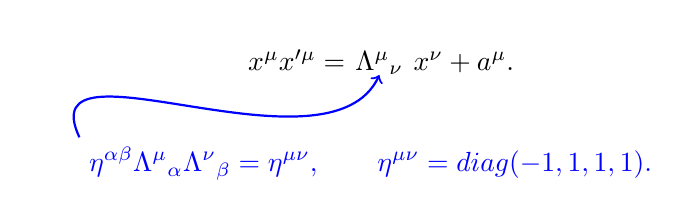
\begin{tikzpicture}[every node/.style={font=\normalsize}]
  \node[anchor=base east] (transform) at (-0.2,0)
    {$x^\mu\rightsquigarrow x'^\mu=$};
  \node[anchor=base west,inner sep=0pt] (lambda) at (transform.base east)
    {$\Lambda^\mu{}_{\nu}$};
  \node[anchor=base west] at (lambda.base east) {$x^\nu+a^\mu.$};
  \node[text=blue,anchor=north] (metric) at (0,-0.85)
    {$\displaystyle
      \eta^{\alpha\beta}\Lambda^\mu{}_{\alpha}\Lambda^\nu{}_{\beta}
      =\eta^{\mu\nu},\qquad
      \eta^{\mu\nu}=\operatorname{diag}(-1,1,1,1).$};
  \draw[blue,->,line width=0.8pt]
    (metric.north west) to[out=115,in=-115] (lambda.south);
\end{tikzpicture}
\end{center}

\YinLine{In QM, represented by a}
\YinIndent{unitary operator \quad $U(\Lambda,a)$. \quad such that}
\[
  \hat\phi(\Lambda x+a)
  =U(\Lambda,a)\,\hat\phi(x)\,(U(\Lambda,a))^{-1}.
\]

\YinLine{It suffizes to study infinitesimal version}
\begin{center}
\begin{tikzpicture}[every node/.style={font=\normalsize}]
  \node[anchor=base east] (lambdaeq) at (0,0)
    {$\Lambda^\mu{}_{\nu}=\delta^\mu{}_{\nu}+$};
  \node[anchor=base west,inner sep=0pt] (omega) at (lambdaeq.base east)
    {$\omega^\mu{}_{\nu},$};
  \node[anchor=base west] (aeq) at (omega.base east) {$\qquad a^\mu=$};
  \node[anchor=base west,inner sep=0pt] (epsilon) at (aeq.base east)
    {$\epsilon^\mu.$};
  \node[text=blue,align=center,below=9mm of omega,xshift=18mm] (small)
    {small, keep only $1^{\mathrm{st}}$ order};
  \draw[blue,->,line width=0.8pt]
    (omega.south) to[out=-80,in=145] (small.north west);
  \draw[blue,->,line width=0.8pt]
    (epsilon.south) to[out=-100,in=35] (small.north east);
\end{tikzpicture}
\end{center}

\begin{center}
\begin{tikzpicture}[every node/.style={font=\normalsize}]
  \node[anchor=base east] (ulead) at (0,0)
    {$U(\Lambda,a)=1-i\epsilon^\mu$};
  \node[anchor=base west,inner sep=0pt] (pgen) at (ulead.base east)
    {$\hat P_\mu$};
  \node[anchor=base west] (umid) at (pgen.base east)
    {$+\dfrac{i}{2}\omega_{\mu\nu}$};
  \node[anchor=base west,inner sep=0pt] (jgen) at (umid.base east)
    {$\hat J^{\mu\nu}.$};
  \node[text=blue,below=11mm of pgen,xshift=-8mm] (plabel)
    {energy-momentum};
  \node[text=blue,align=center,below=11mm of jgen,xshift=8mm] (jlabel)
    {boost\\$+$ angular\\momentum};
  \draw[blue,->,line width=0.8pt]
    (plabel.north) to[out=80,in=-110] (pgen.south);
  \draw[blue,->,line width=0.8pt]
    (jlabel.north) to[out=100,in=-70] (jgen.south);
\end{tikzpicture}
\end{center}

% These four lines are faint gray marginalia in the source.
\YinGray{%
\[
  U(\Lambda',a')U(\Lambda,a)
  =U(\Lambda'\Lambda,\Lambda'a+a').
\]
\[
  [P,P]=0.
\]
\[
  [P^\mu,J^{\rho\sigma}]
  =-i\bigl(\eta^{\mu\rho}P^\sigma-(\rho\leftrightarrow\sigma)\bigr).
\]
\[
  [J^{\mu\nu},J^{\rho\sigma}]
  =-i\bigl(\eta^{\nu\rho}J^{\mu\sigma}
            -\eta^{\mu\rho}J^{\nu\sigma}
            -(\rho\leftrightarrow\sigma)\bigr).
\]
}

% ---------------------------------------------------------------------------
\YinPageBoundary{7}{12}

\YinLine{Micro causality;}
\[
  [\hat\phi(x),\hat\phi(y)]=0
  \qquad
  \begin{gathered}
    \text{whenever $x,y$}\\
    \text{are spacelike}\\
    \text{- separated.}
  \end{gathered}
\]
\YinIndent{i.e.}
\[
  (x-y)^2\equiv-(x^0-y^0)^2+(\vec x-\vec y)^2
\]
\[
  >0.
\]

\YinBullet{What about our model of}
\YinIndent{\hspace*{1.4em}free relativistic particles?}
\[
  H=\int d^{D-1}\vec p\,
  \sqrt{\vec p^{\,2}+m^2}\,
  a_{\vec p}^{+}a_{\vec p},
\]
\[
  \vec P=\int d^{D-1}\vec p\,
  \vec p\,a_{\vec p}^{+}a_{\vec p}.
\]
\[
  \hat P^\mu=(H,\vec P).
\]

\YinLine{Does $\hat\phi(x)$ exist? \qquad Yes!}
\[
  \hat\phi(x)=
  \int\frac{d^{D-1}\vec p}
  {\sqrt{(2\pi)^{D-1}2\omega_{\vec p}}}
  \left(
    a_{\vec p}
    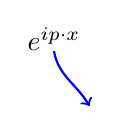
\begin{tikzpicture}[baseline=(positivephase.base)]
      \node[inner sep=0pt] (positivephase) {$e^{ip\cdot x}$};
      \draw[blue,->,line width=0.8pt]
        (positivephase.south) to[out=-80,in=120] (0.45,-0.85);
    \end{tikzpicture}
    +a_{\vec p}^{+}e^{-ip\cdot x}
  \right)
\]

% ---------------------------------------------------------------------------
\YinPageBoundary{8}{13}

\begin{center}
\begin{tikzpicture}[every node/.style={font=\normalsize}]
  % U13-1: the separate opening curve is visible but has no assigned meaning.
  \draw[blue,line width=0.8pt] (-3.2,0.25) to[out=110,in=-115] (-2.85,1.0);
  \node[text=blue,align=left] (definitions) at (1.25,0)
    {$\begin{aligned}
       p\cdot x&\equiv\vec p\cdot\vec x-\omega_{\vec p}x^0.\\
       \omega_{\vec p}&\equiv\sqrt{\vec p^{\,2}+m^2}.
     \end{aligned}$};
  \draw[blue,->,line width=0.8pt]
    (-2.5,0.9) to[out=-115,in=175] (definitions.west);
\end{tikzpicture}
\end{center}

\YinLine{Check micro causality;}
\[
  [\hat\phi(x),\hat\phi(y)]
  =\int\frac{d^{D-1}\vec p}{(2\pi)^{D-1}2\omega_{\vec p}}
  \cdot
  \left[e^{ip\cdot(x-y)}-e^{-ip\cdot(x-y)}\right]
\]
% AMBIGUITY A8-1: the source appears to write d^D p^\mu. See ambiguities.md.
\[
  =\int
  \underbrace{%
    \frac{d^D p^\mu}{(2\pi)^{D-1}}
    \theta(p^0)\delta(p^2+m^2)
  }_{\YinBlue{\substack{\text{invariant under}\\p^\mu\to\Lambda^\mu{}_{\nu}p^\nu}}}
  \underbrace{%
    \left[e^{ip\cdot(x-y)}-e^{-ip\cdot(x-y)}\right]
  }_{\YinBlue{\substack{\text{inv't under}\\
                         x\to\Lambda x,\ y\to\Lambda y.}}}
\]
\begin{center}
  \YinBlue{result a function of $(x-y)^2$ only.}
\end{center}

\YinLine{If $(x-y)^2>0$, WLOG can take $x^0-y^0=0$.}
\YinLine{\hfill $\vec x-\vec y\ne0$.\hspace*{7em}}
\YinLine{integrand odd under $\vec p\to-\vec p$}
\YinLine{\hspace*{4em}thus $\displaystyle\int\cdots=0$,}
\YinLine{i.e. \quad $[\hat\phi(x),\hat\phi(y)]=0$ for $(x-y)^2>0$.
  \quad\YinBlue{$\checkmark$}}

% ---------------------------------------------------------------------------
\YinPageBoundary{9}{14}

\YinBullet{Can also verify that}
\[
  U(\Lambda,a)\,\hat\phi(x)\,(U(\Lambda,a))^{-1}
  =\hat\phi(\Lambda x+a).
\]

% U14-1: the two terminal marks are preserved as shapes without prose meaning.
\noindent
\begin{tikzpicture}[baseline]
  \draw[-{Stealth[length=2.2mm,width=1.7mm]},line width=0.45pt]
    (0,0) -- (0.92\linewidth,0);
  \node[anchor=west,inner sep=1pt,font=\scriptsize] at (0.925\linewidth,0)
    {{}''};
\end{tikzpicture}\par

\bigskip
\YinLine{Postulate that the properties}
\YinBullet{Hilbert space $\mathcal H$}
\YinBullet{Poincar\'e sym $U(\Lambda,a)$}
\YinBullet{Poincar\'e - invt vacuum $\ket{\Omega}$}
\YinBullet{local ``field'' operators \quad $\hat\phi(x)$}
\YinIndent{\hspace*{1.4em}that obey Poincar\'e - covariance and}
\YinIndent{\hspace*{9em}microcausality.}

\YinIndent{hold for system of interacting}
\YinIndent{relativistic particles as well!}

\bigskip
\YinDash{How to construct such theories~?}
\YinDash{useful to work with a formalism in}
\YinIndent{\hspace*{1.4em}which Poincar\'e sym is manifest.}
